\documentclass{article}
\usepackage[utf8]{inputenc}


\usepackage[lined, boxed, linesnumbered]{algorithm2e}
\usepackage{natbib}
\usepackage{amsfonts}
\usepackage{amsthm}
\usepackage{float}
\usepackage{mathtools}
\usepackage{graphicx}
\usepackage{multicol}
\usepackage{blindtext}
\usepackage[top=2cm, bottom=2cm, left=2cm, right=2cm]{geometry}
\usepackage{fancyhdr}

\bibliographystyle{apalike}

\newtheorem{theorem}{Theorem}[section]
\newtheorem{corollary}{Corollary}[theorem]
\newtheorem{lemma}[theorem]{Lemma}


%%%%%%%%%%%%%%%%%%%%%%%%%%%%%% FANCY HEADER %%%%%%%%%%%%%%%%%%%%%%%%%%%%%%%%%%%
\fancyhead{}
\fancyfoot{}
\fancyhead[C]{\bf Temporal Networks with Resource Constraints.}
\renewcommand{\headrulewidth}{1pt}
\newcommand{\HRule}{\rule{\linewidth}{0.5mm}}

%%%%%%%%%%%%%%%%%%%%%%%%%%%%%% DOCUMENT %%%%%%%%%%%%%%%%%%%%%%%%%%%%%%%%%%%%%%%

\begin{document}
\thispagestyle{empty}

\begin{center}
%%%%%%%%%%%%%%%%%%%%%%%%%%%%%% TITLE PAGE %%%%%%%%%%%%%%%%%%%%%%%%%%%%%%%%%%%%%
\HRule \\[0.3cm]
{\Large \bfseries
Temporal Networks with Resource Constraints\\[0.3cm]}
\HRule \\[0.5cm]

\noindent
\begin{minipage}{0.5\textwidth}
\begin{flushleft}
\textbf{Szymon Sidor\\
Peng Yu\\
Cheng Fang\\
Brian Williams}\\
Massachusetts Institute of Technology
\end{flushleft}
\end{minipage}%
\begin{minipage}{0.5\textwidth}
\begin{flushright}
\textsc{sidor@mit.edu}\\
\textsc{yupeng@mit.edu}\\
\textsc{cfang@mit.edu}\\
\textsc{williams@mit.edu}\\
$\ $
\end{flushright}
\end{minipage}
\\[1cm]
\end{center}
\pagestyle{fancy}

\begin{multicols}{2}
%%%%%%%%%%%%%%%%%%%%%%%%%%%%%% ABSTRACT %%%%%%%%%%%%%%%%%%%%%%%%%%%%%%%%%%%%%%%
\begin{abstract}
\noindent %\blindtext
\end{abstract}
%%%%%%%%%%%%%%%%%%%%%%%%%%%%%% INTRODUCTION %%%%%%%%%%%%%%%%%%%%%%%%%%%%%%%%%%%
\section{Introduction}
%\blindtext[5]

%%%%%%%%%%%%%%%%%%%%%%%%%%%%%% RELATED WORK %%%%%%%%%%%%%%%%%%%%%%%%%%%%%%%%%%%
\section{Related Work}
%\blindtext[5]

One of the earliest mentions of a scheduling problem being solved in an algorithmic fashion can be found in \cite{johnson1954optimal}, although there's evidence that the problem was already considered in unpublished versions of \cite{bellman1956mathematical}. This publication considers the following statement of scheduling problem. We have $n$ items and $m$ stages and $A_{i,j}$ denoting the time for $i$-th item to be processed by stage $j$. All the items must be processed by different stages in order (for example first stage is printing of a book and second stage is binding). The publication considers $m=2$ and $m=3$ and arrives at the solution that \textit{``permits one to optimally arrange twenty production items in about five minutes by visual inspection''}. It turns out that the solution to the problem for $m \geq 3$ is NP-hard (\cite{garey1976complexity}). In \cite{wagner1959integer} an Integer Programming solution to the scheduling problem and noticed that it \textit{``is a single model which encompasses a wide variety of machine-scheduling situations''}.

In \cite{pritsker1969multiproject} a generalization of scheduling problem is considered, which allows for multiple resource constraints. However the solution provided uses a discrete time formulation, which depending on required accuracy can substantially decrease performance. Work in this publication considers work on Temporal Networks, which explictly model continuous time constraints. In \cite{dechter1991temporal} a notion of Simple Temporal Problem was introduced which allows one to solve problem with simple temporal constraints of form $l \leq t_y - t_x \leq u$. This simple concept was later extended with various more sophisticated notions of temporal constraints. \cite{vidal1996dealing} defined the notion of uncertain temporal constraint, where the duration between two time events can take a value from an interval $[l,u]$ which is unknown during the time of scheduling (uncertain duration constraints); consistency of such temporal networks is called Strong Controllability. \cite{morris2001dynamic} desribes a pseudopolynamial algorithm for handling uncertain duration constraint, where we are allowed to make a descition scheduling decitions based on knowledge of uncertain durtions from the past (Dynamic controllability). His algorithm is later improved to polynamial complexity (\cite{morris2005temporal}). Finally, \cite{Fang2014} provides a non-linear optimization based solver for uncertain temporal constraints where the duration of the constraint can come from abritrary probabilistic distribution.

%%%%%%%%%%%%%%%%%%%%%%%%%%%%%% PROBLEM STATEMENT %%%%%%%%%%%%%%%%%%%%%%%%%%%%%%
\section{Problem statement}
In this section we will define notion of a Time Resource Network (TRN) and the relevant constraint on TRN's schedule - Resource Consistency. All the results presented in this paper scale to multiple different type of resources being constraint at the same time (electricity, water, fuel, cpu time, memory etc.), but to simplify the notation we will assume that only one type of resource is constrained.
\subsection{Abstract Temporal Network}
Since TRNs can operate on top of many different types of temporal networks, we define a notion of Abstract Temporal Network (ATN), to capture only the necessary properties. For abstract temporal network we define two pieces of functionality:
\begin{enumerate}
\item \texttt{nodes(ATN)}, which returns a set of timepoints in $ATN$
\item \texttt{extend(ATN, $\{ stc_1, ... stc_n \} $)}, which takes ATN and set of simple temporal constraints \cite{cervoni1993maintaining} spanning \texttt{nodes(ATN)}, and returns another $ATN'$, such that there exists a schedule satisfying $p-TC(ATN')$ if and only if there exists a schedule satisfying $p-TC(ATN)$ and the obeying set of simple temporal constraint $\{ stc_1, ... stc_n \} $. $p-TC$ is a notion of probabilistic temporal consistency described in section \ref{temporal_consistency}.
\end{enumerate}
As the following section describes in detail we will use \texttt{extend} to encode resource constraints over \texttt{nodes}.
\subsection{Temporal Consistency}
\label{temporal_consistency}
For an ATN we define a predicate $TC(ATN)$. $TC$ is true if we can find acceptable execution strategy for that network (what that means precisely depends on the ATN - we only require for it to be verifiable).
\paragraph{Example} Let's consider cc-pSTP \cite{Fang2014} as an example. Here \texttt{nodes} returns set of \textit{activated} and \textit{received} timepoints. \texttt{extend} returns network with extra \textit{free contraints} encoding the simple temporal constraints. The temporal consistency check $TC$ is true if cc-pSTP has a solution.
\subsection{Time Resource Network}
A Time Resource Network $TRN = (ATN, {rc_1, ..., rc_n})$, where $ATN$ is an Abstract Temporal Network and ${rc_1, ..., rc_n}$ is a set of resource constraints. There are a few different types of resource constraints, but they all have a common property - they describe resource usage between two timepoints in \texttt{nodes(ATN)}.
\subsection{Schedule}
A schedule $s: \texttt{nodes(ATN)} \rightarrow \mathbb{R}$ is a mapping from abstract timepoints in ATN to concrete execution times.
\subsection{Resource constraints}
\begin{itemize}
\item \textbf{simple resource constraint} is a triplet $(x, y, r)$, where $x, y \in$ \texttt{nodes(ATN)} and $r$ is resource usage which can be positive (consumption) and negative (generation). For any time $s(x) \leq t \leq s(y)$ usage is equal to
\[
u(t) = r
\]
Where $s$ is a schedule. Intuitively, simple resource constraint encodes the fact that between time $s(x)$ and $s(y)$  resource is consumed (generated) at the rate $|r$| units of resource per unit time for positive (negative) $r$.
\item \textbf{linear resource constraint} is a triplet $(x, y, r_b, r_e)$, where $x, y \in \texttt{nodes(ATN)}$ and resource usage at time $s(x) \leq t \leq s(y)$ is equal to
\[
    u(t) = r_b + t  \frac{r_e - r_b}{s(y) - s(x)}
\]
Intuitively, simple resource constraint encodes the fact that between time $s(x)$ and $s(y)$  resource is consumed/generated with rate that changes linearly between $s(x)$ and $s(y)$.
\item \textbf{probabilistic simple resource constraint}
Is an extension of simple resource constraint where $r$ is a random variable (and therefore so is $u(t)$).
\item \textbf{probabilistic linear resource constraint}
Is an extension of simple resource constraint where $r_b$ and $r_e$ are a random variables (and therefore so is $u(t)$).
\end{itemize}
Notice in particular that all the resource constraints are special cases of probabilistic linear resource constraint. Indeed, constant functions family is a subset of linear function family and the non-probabilistic versions of constraints can be though of as Dirac delta function probability distributions.

\paragraph{Example} Describe solar panel example.


\subsection{$p$-Resource consistency}
For a given schedule $s$ let's define random variable $U_s(t)$ as net usage of the resource at time $t$ under schedule $s$. More formally
\[
U_s(t) = \sum_{\forall_{(x_i,y_i,u_i) \in R}. s(x_i)\leq t \leq s(y_i)} u_i(t)
\]
Where $R$ is a set of all the resource constraints and $x_i$, $y_i$ and $u_i$ are as described in section about linear resource constraints ($r_b$ and $r_e$ are encapsulated by $u$). We say the network satisfy the network is \textbf{$p$-resource consistent} under schedule $s$ if it newer uses more resources than limit, i.e.
\[
\forall_{r \in R} \forall_{t} . U_s(t) \leq 0
\]
with probability $p$. When dealing with the special case of non-probabilistic duration we drop the $p$ and talk about \textbf{resource-consistency} as for any non-zero value of $p$ the outcome is the same.

\subsection{Time-resource consistency}
The problem that we are solving in this paper is determining whether TRN is time-resource consistent. Before defining exactly what this means we prove the following lemma:

\begin{lemma}
\label{resource_checking}
Assume we have a TRN, such that ATN has explicit timepoints for start and end of the time horizon (can be $\pm \infty$).
A schedule is resource-consistent if and only if
\[
\forall_{t \in \texttt{nodes(ATN)}} U_s(s(t)) \leq 0
\]
i.e. resource usage is not non-positive at all of the scheduled timepoints.
\end{lemma}
\begin{proof}
$\Rightarrow$ Trivial from definition of resource-consistency.
$\Leftarrow$ We say a time $t \in \mathbb{R}$ is scheduled if there exists a timepoint  $x \in \texttt{nodes(ATN)}$ such that $t = s(x)$. We can rephrase right side of the lemma saying that for all the scheduled $t$ $U_s(t) \leq 0$. Assume that the right side of the implication is satisfied but the schedule is not resource consistent. That means that there exists a time point $t_{danger}$ which is not schduled for which $U_s(t_{danger}) > 0 $. Let $x$ be highest scheduled time less than $t_{danger}$ and let $y$ be smallest scheduled time higher than $t_{danger}$. We know that $U_s(t)$ for $x \leq t \leq y$ is a sum of linear functions (or possibly zero), which is itself a linear function. This means that either $U_s(x) \geq t_{danger}$ or $U_s(y) \geq t_{danger}$, so either $U_s(x) > 0$ or $U_s(y) > 0$. But both $x$ and $y$ are scheduled. Contradiction.

\end{proof}
\begin{corollary}
Given a $TRN$ with only simple resource constraints and two schedules $A$ and $B$ that have the same ordering of timepoints, $A$ is $p$-resource-consistent if and only if $B$ is $p$-resource-consistent.
\end{corollary}
\begin{proof}
Notice that if we move arbitrary timepoint, while preserving the relative ordering of timepoints, then net resource usage at that timepoint will not change (as the $U_s(t)$ between the neighboring timepoints remains constant). Therefore by lemma \ref{resource_checking} we can transform schedule $A$ into schedule $B$.
\end{proof}
Notice that the Corollary does not apply to the linear resource constraints (see fig. TODO).

TODO: generalize to probabilistic

Finally we say that a TRN is \textbf{$p$-time-resource consistent} if there exists and ordering of timepoints such that every schedule that satisfies this ordering is $p$-resource-consistent and $ATN$ extended with that ordering is $TC$.

%%%%%%%%%%%%%%%%%%%%%%%%%%%%%% ALGORITHM %%%%%%%%%%%%%%%%%%%%%%%%%%%%%%%%%%%%%%
\section{Algorithm}
High level idea of the algorithm is quite simple and is presented in algorithm \ref{hl_algo}. In the second line we iterate over all the permutations of the timepoints. On line 3 we use \texttt{p\_resource\_consistent} function to check resource consistency, performing this check is the nontrivial part of the algorithm. On line four we use $TC$ checker to determine if network is time consistent - the implementation depends on $ATN$ and we assume it is available. Function $encode\_as\_scts$ encodes permutation using simple temporal constraints. For example if $\sigma(1) = 2$ and $\sigma(2) = 1$ and $\sigma(3) = 3$, then we can encode it by two STCs: $ 2 \leftarrow 1 $ and $1 \leftarrow 3$.

\begin{algorithm}[H]
    \label{hl_algo}
    \KwData{TRN and p}
    \KwResult{true if TRN=(ATN, RC) is p-time-resource-consistent}
    $N \leftarrow \texttt{nodes(ATN)}$\;
    \For{$\sigma \leftarrow \text{permutation of } N$}{
        \If{\texttt{p\_resource\_consistent(RC, $\sigma$, $p$)} }{
            \If{TC(\texttt{extend(ATN, encode\_as\_scts($\sigma$))})}{
                succeed\;
            }
        }
    }
    fail\;
    \caption{Checking $p$-time-resource-consistency of a TRN }
\end{algorithm}
Implementation of \texttt{p\_resource\_consistent} follows from lemma \ref{resource_checking}.



% INPUT: atn N, {src} S (spanning N.timepoints)
% OUTPUT: scheduling strategy on N or fail
% ALGORITHM:
% X = subset of N.timepoints used by SRCs from S
% for every permutation pi of X:
% stcs = pi encoded by STCs
% result = N.solve_with_stcs(stcs)
% if result is schedule:
%        return schedule
%       fail



%%%%%%%%%%%%%%%%%%%%%%%%%%%%%% EXPERIMENTS %%%%%%%%%%%%%%%%%%%%%%%%%%%%%%%%%%%%
\section{Experiments}

\subsection{TRN over pSTN}
To demonstrate extensibility of our approach we have implemented a version of TRN network, where the underlying temporal network is pSTN (\cite{Fang2014}). pSTN extends the notion of STN. For this discussion we define STN nodes and edges as \textbf{actiavated time points} and \textbf{free constraints} respectively. pSTN defines \textbf{received time point} which is determined by the environment. Every received time point is defined by corresponding \textbf{uncertain duration (uDn)} constraint, which specifies a probability distribution over duration between an activated time point and a received time point. Due to that extension, the notion of consistency becomes probabilistic; rather than asking \textit{is this pSTN consistent?}, we ask is \textit{is this pSTN consistent with probability $p$?}. Since pSTN is an extension of STN, it is an ATN.

Let's consider the following Smart House scenario. We have $150W$ generator which is available. We know that the user comes back from work at some time defined by a gaussian distribution $N(5pm, 5m)$. Moreover we know that sun sets at time defined by $N(7pm, 1m)$. We would like to meet the following constraints with the overall probability at least $98\%$:
\begin{itemize}
\item Wash clothes (duration: $2h$, power usage: $130W$) before user comes back from work
\item Cook dinner (duration: $30m$, power usage: $100W$) ready within 15 minutes of user coming back from work
\item Have the lights on (power usage: $80W$) from before sunset to at least midnight.
\item Cook a late night snack (duration: $30m$, power usage: $20W$) between 10pm and 11pm.
\end{itemize}

Our algorithm succesfully finds a solution to this scenario which meets the constraints with $p=$.  It is presented on fig. \ref{fig:pstnu_scheduling}.

\begin{figure}[H]
\begin{center}
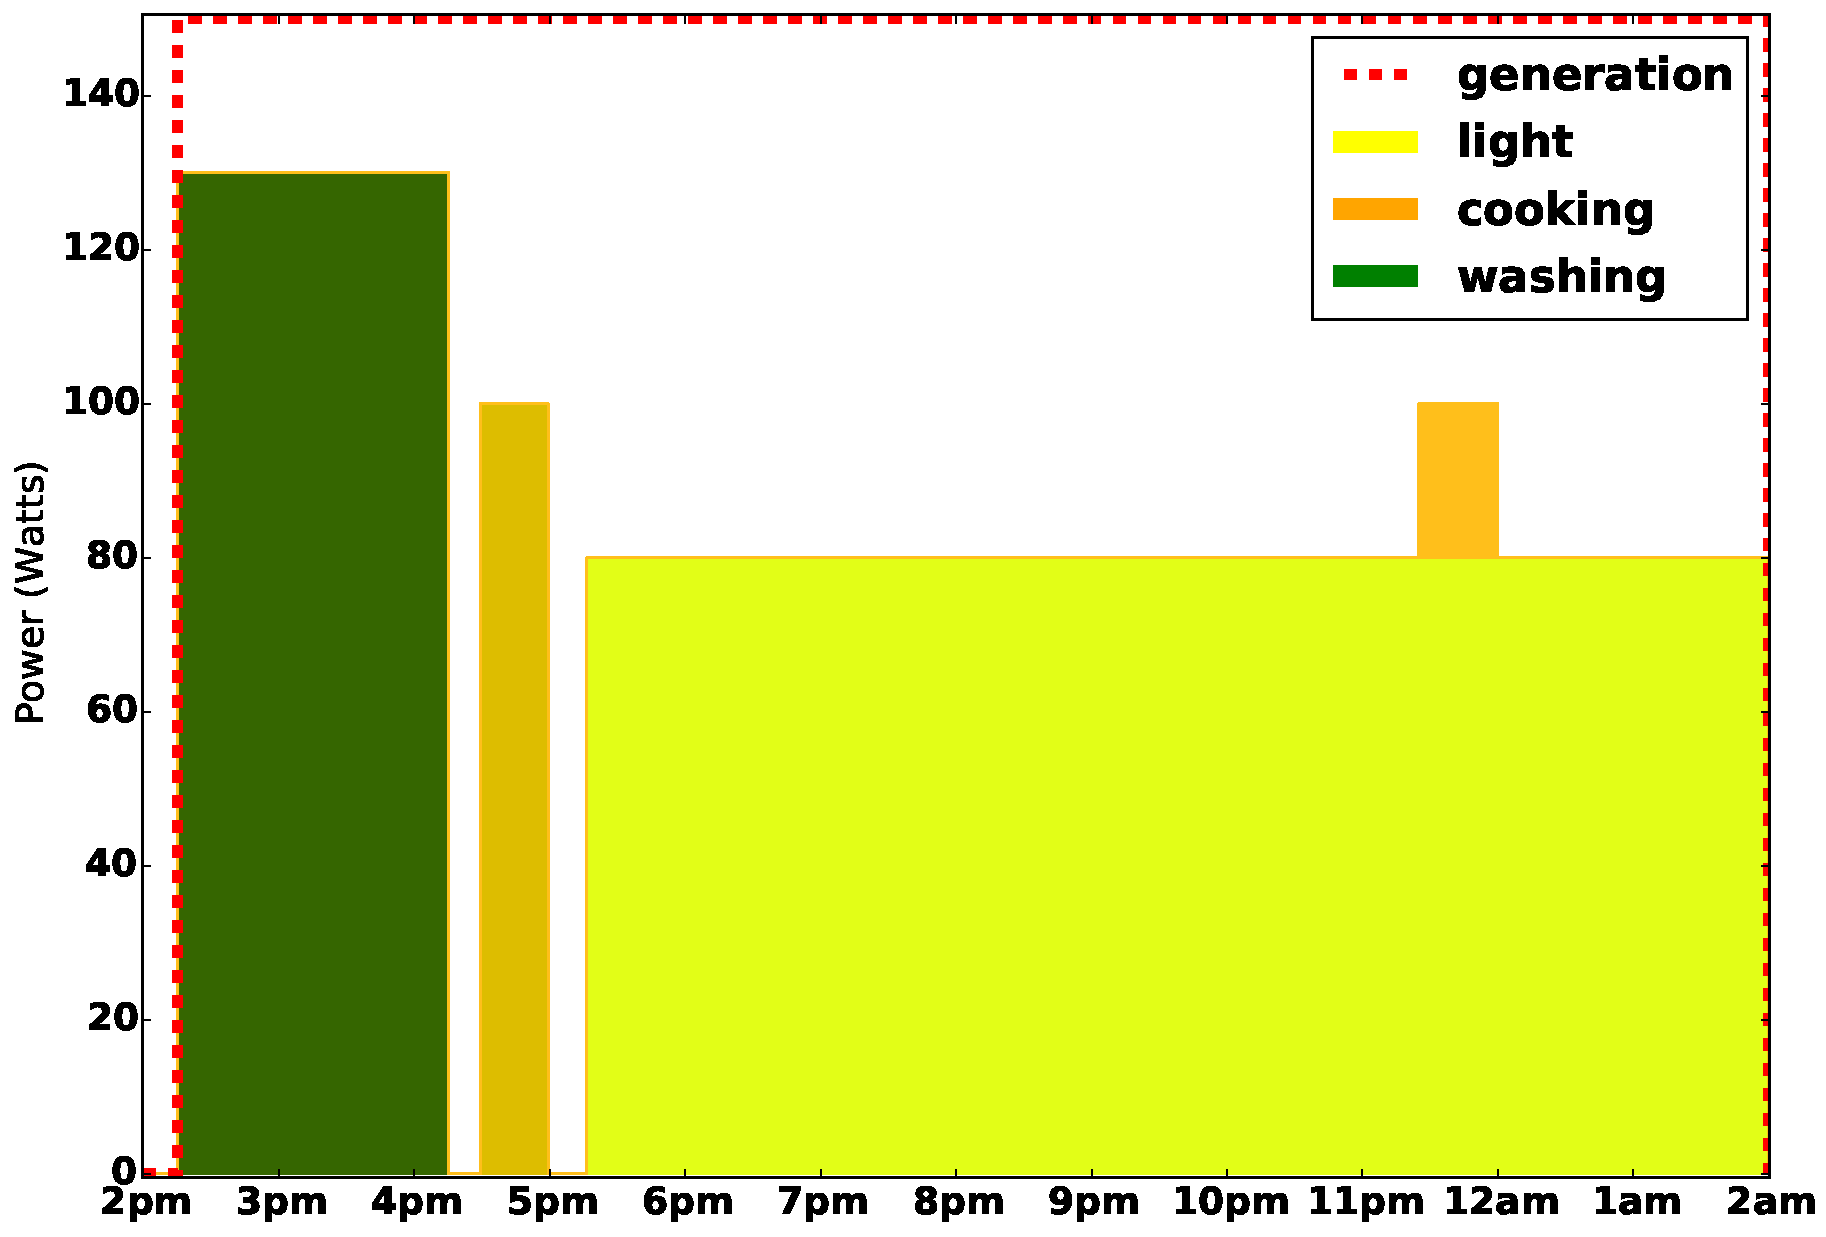
\includegraphics[width=0.49\textwidth]{../pstnu_scheduling}
\caption{Depiction of solution to TRN spanning a pSTN.}
\label{fig:pstnu_scheduling}
\end{center}
\end{figure}




%%%%%%%%%%%%%%%%%%%%%%%%%%%%%% FUTURE WORK %%%%%%%%%%%%%%%%%%%%%%%%%%%%%%%%%%%%
\section{Future Work}
%%%%%%%%%%%%%%%%%%%%%%%%%%%%%% CONCLUSION %%%%%%%%%%%%%%%%%%%%%%%%%%%%%%%%%%%%%
\section{Conclusion}
%\blindtext[5]
%%%%%%%%%%%%%%%%%%%%%%%%%%%%%% REFERENCES %%%%%%%%%%%%%%%%%%%%%%%%%%%%%%%%%%%%%
\section{References}

\bibliography{references}
\end{multicols}
\end{document}
